\documentclass[11pt, a4paper]{article}

\usepackage{anyfontsize}
\usepackage{txfonts} 
\usepackage{booktabs}
\usepackage{array}
\usepackage{geometry}
\usepackage{lscape}
\usepackage{graphicx}
\graphicspath{{img/}}
\geometry{left=3cm,right=2.5cm,top=3.5cm,bottom=4cm}

%Graphics preamble
\usepackage{graphicx} %Allow you to import images
\usepackage{float} %Allow for control of float position

%Header and Footer Stuff
\pagestyle{myheadings}\markboth{page \thepage}{\emph Software Engineering and Project
Software Project Management Plan}

%Table
\setlength{\arrayrulewidth}{0.5mm}

\begin{document}

\begin{titlepage}

\begin{center}

	\vspace{0.5 cm}
	\fontsize{35}{35}\selectfont\bf {Software Engineering and Project
Software Project Management Plan}\\
	
	
	\vspace{2cm}
	\Large\textbf{ Version 2.0 approved}\\
	
	\vspace{1.5cm}
	\Large\textbf {Prepared by SEP Group 19 - Spark\\
								Luo Yawen a1657343 \\
								Wei Jingwen a1671836 \\
								Wang Yuzhu a1690773 \\
								Yang Jiajun a1662541\\
								Zhang Yun a1653772}\\
		
	\vspace{2cm}
	\Large\textbf{ School of Computer Science,\\
								The University of Adelaide}\\
	\vspace{2cm}
	
	\Large\textbf{ Nov 01, 2015}\\

\end{center}

\end{titlepage}

%This is table of contents stuff
\pagenumbering{roman}
\tableofcontents

%This is the version history stuff
\vspace{1cm}
\section*{Revision History}
\addcontentsline{toc}{section}{\numberline{}Revision History}
%\begin{table}
\small
\begin{tabular} 
	 {|m{3cm}|m{2cm}|m{8cm}|m{2cm}|}
	\hline
	\textbf{Name} &  \textbf{Date} & \textbf{Reason For Changes} & \textbf{Version} \\ [0.5ex]
	\hline
	Wang Yuzhu & 02/Sep/15 & Add section 1.1 \& 1.2 & 0.1 \\ [0.5ex]
	\hline
	Wang Yuzhu & 03/Sep/15 & Add section 1.3 \& 1.4 & 0.2 \\ [0.5ex]
	\hline
	Wang Yuzhu & 04/Sep/15 & Add section 2 \& 3 & 0.3 \\ [0.5ex]
	\hline
	Wang Yuzhu & 05/Sep/15 & Add section 4.1 \& 5.1 & 0.4 \\ [0.5ex]
	\hline
	Wang Yuzhu & 06/Sep/15 & Add section 5.2 \& 5.3 \& 5.4 & 0.5 \\ [0.5ex]
	\hline
        Wang Yuzhu & 07/Sep/15 & Add section 6 & 0.6 \\ [0.5ex]
	\hline
	Luo Yawen & 08/Sep/15 & Add section 7.1 \& 7.2 & 0.7 \\ [0.5ex]
	\hline
	Luo Yawen & 09/Sep/15 & Add section 7.3 \& 7.4  & 0.8 \\ [0.5ex]
	\hline
	Yang Jiajun & 09/Sep/15 & Add section 8 & 0.9 \\ [0.5ex]
	\hline
	Luo Yawen & 9/Oct/15 & Release & 1.0 \\ [0.5ex]
	\hline
	Wang Yuzhu & 05/Oct/2015 & Update section 1-3 & 1.3 \\ [0.5ex]
	\hline
	Wang Yuzhu & 07/Oct/2015 & Update section 4 & 1.4 \\ [0.5ex]
	\hline
	Wang Yuzhu & 08/Oct/2015 & Update section 5 & 1.5\\ [0.5ex]
	\hline
	Wang Yuzhu & 09/Oct/2015 & Update section 6 & 1.6 \\  [0.5ex]
	\hline
	Yang Jiajun & 10/Oct/2015 & Update section 8 & 1.7 \\ [0.5ex]
	\hline
	Luo Yawen & 11/Oct/2015 & Update section 7 & 1.8\\ [0.5ex]
	\hline
	Luo Yawen \newline  Wang Yuzhu \newline Yang Jiajun & 15/Oct/15 & Review & 1.9 \\ [0.5ex]
	\hline
	Luo Yawen & 01/Nov/15 & Final release & 2.0 \\ [0.5ex]
	\hline
		
\end{tabular}
%\end{table}
\cleardoublepage

\newpage


%This is main body stuff
\pagenumbering{arabic}
\setcounter{page}{1}

%section1
\section{Introduction}
\subsection{Purpose and Scope}
The purpose of this system is to design a Lego Mind storms EV3 robot which will be used to find markings in a survey area, a single A1 sized paper, and work from these markings to make a map to show the location of these markings. The system does not need to develop hardware (the robot) as it has been provided. In addition, the system needs to deliver documents, including SRS, SPMP, SDD, User Manual and Test Report to the client.

\subsection{Assumptions and constraints}
The development team works in a small company. The team will have a short meeting with the client each week to ask questions and work out the requirements. Also, the team will have group meetings without the client over the development process that discuss the develop schedule and unsolved problems. Requirement changes will constraint the progress of development.

\subsection{Project deliverables}
In this project there are 8 deliveries need to be derived, each delivery must be committed to the SVN before the due time. Any commits after the due time will not be considered. 

%Here we insert our figure
\begin{figure}[H]
\centering
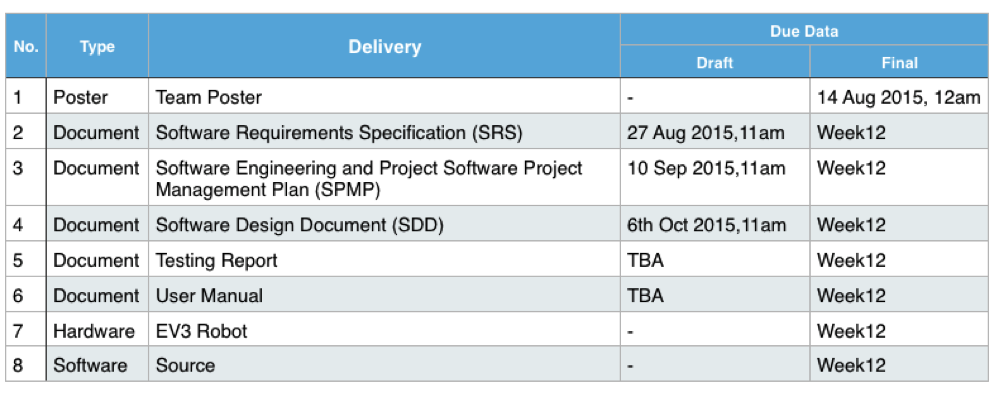
\includegraphics[height=2.5in]{PD.png}
\caption[Project deliverable]{Project deliverable}
\end{figure}

\subsection{Evolution of the plan}
\begin{itemize}
\item{\bfseries Initial Description}\\
The first sketch of the Mesa Mapping Robot was planned at the first group meeting in August 2015. Over the first group meeting, team members' roles and responsibilities were discussed. After the second meeting with the client the team made a development schedule based on the course plan and listed the requirements of the client that the robot will be used to find markings on a survey map to make map.
\item{\bfseries Develop Alternatives}\\
After the third time group meeting, two development alternatives were decided based on the client requirements, the provided hardware and team member's strength and weakness. The two alternatives are all focus on developing stable robot and making an accurate map. Each of the alternative is described below.
\item{\bfseries Alternative A - Wheels Driven Robot}\\
The robot will be designed to be driven by wheels. The distance sensor is designed on the top of the robot and the colour sensor is designed under the robot. Alternative A focuses on the flexibility of the robot.
\item{\bfseries Alternative B - Track Driven Robot}\\
The robot will be designed to be driven by track. The distance sensor and the colour sensor are designed on both arms of the robot. Alternative B focuses on the stability of the robot.
\item{\bfseries Final Draw}\\
Alternative B was chosen, designs and development process were determined, the reason why we choose alternative B is that after we tested both wheels driven robot and track driven robot, we found that track driven robot is more stable, this can increase the stability of the sensor and can help the robot control its body more accurately. In addition, alternative B is more personalised. The meeting will be held with the client weekly and the development schedule will be adjusted according to the requirements change.
\end{itemize}

%section2
\section{References}
Software Requirements Specification (SRS)\\
\\
SVN: https://version-control.adelaide.edu.au/svn/SEPADL15S2PG19/\\
\\
Software Engineering, 9th Edition, Ian Sommerville\\
\\
Software Engineering and Project (2015)\\
https://forums.cs.adelaide.edu.au/pluginfile.php/46004/block\_html/content/ProjectDescription\_2015sem2.pdf\\
\\
https://www.tbs-sct.gc.ca/itp-pti/pog-spg/epd-tbdp/epd-tbdp08-eng.asp\\

%section3
\section{Definitions}
\begin{itemize}
\item {SRS - }Software Requirements Specification\\
\item {SPMP - }Software Project Management Plan\\
\item {SDD - }Software Design Document\\
\item {GUI - }Graphics Users Interface
\end{itemize}
\newpage

%section4
\section{Project organisation}
\subsection{Roles and responsibilities}
The table describes the roles and responsibilities of each member, as well as rationale.
%Here we insert our figure
\begin{figure}[H]
\centering
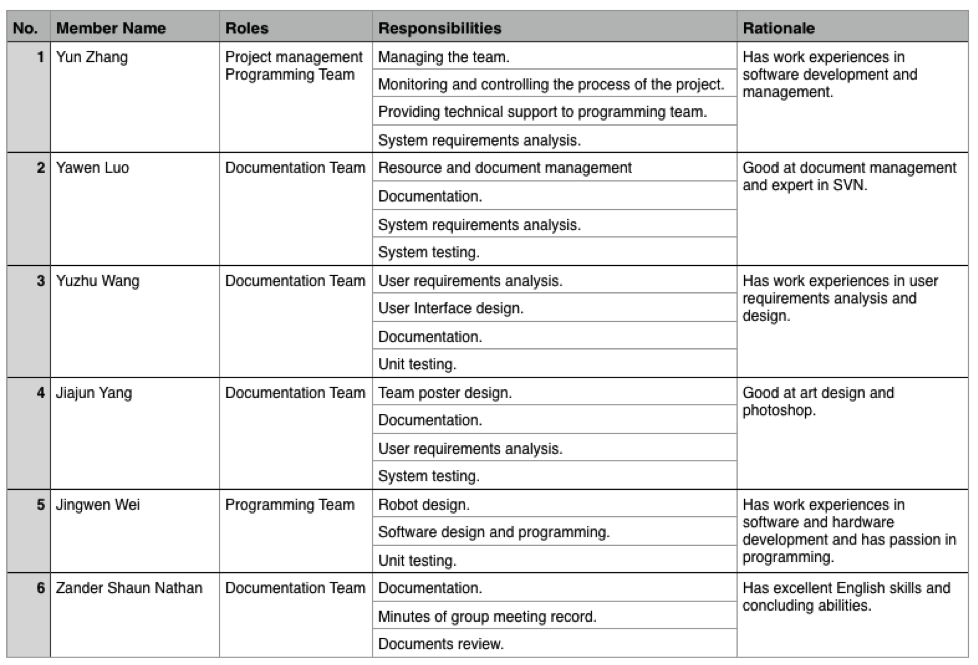
\includegraphics[height=4.5in]{RR.png}
\caption[Roles and responsibilities]{Roles and responsibilities}
\end{figure}

%section5
\section{Risk management plan}
In this section the Risk management plan, including Risk Planning, Risk Identification and Risk Monitoring and Review in the Robot Mapping System will be described. Risk management plan is a very important part over the development process, as it may affect the project schedule or the quality.

\subsection{Risk Planning}
The project manager will ensure that risks are identified, analysed, monitoring and recorded during the whole project. All the risks should be identified and analysed as early as possible to minimise their impact to the project. Each member will be assigned a risk to monitoring that if the risk is becoming more or less possible.\\
\\
Ways to prevent the risk from occurring or reduce its likelihood and impact will be identified by the project team. This may include adjusting project schedule, changing tasks, changing resources and so on.\\

\subsection{Risk Identification and Analysis}
Risk identification will involve the project team, client, and will include the human factors, technical factors and the project management plan. Project deliverables will be carefully assumed, constrained and estimated. Risk management log will be recorded for each risk. All the identified risk will be analysed to determine which risks are high likelihood, high impact and which risks can be prevented from occurring.

%Here we insert our figure
\begin{figure}[H]
\centering
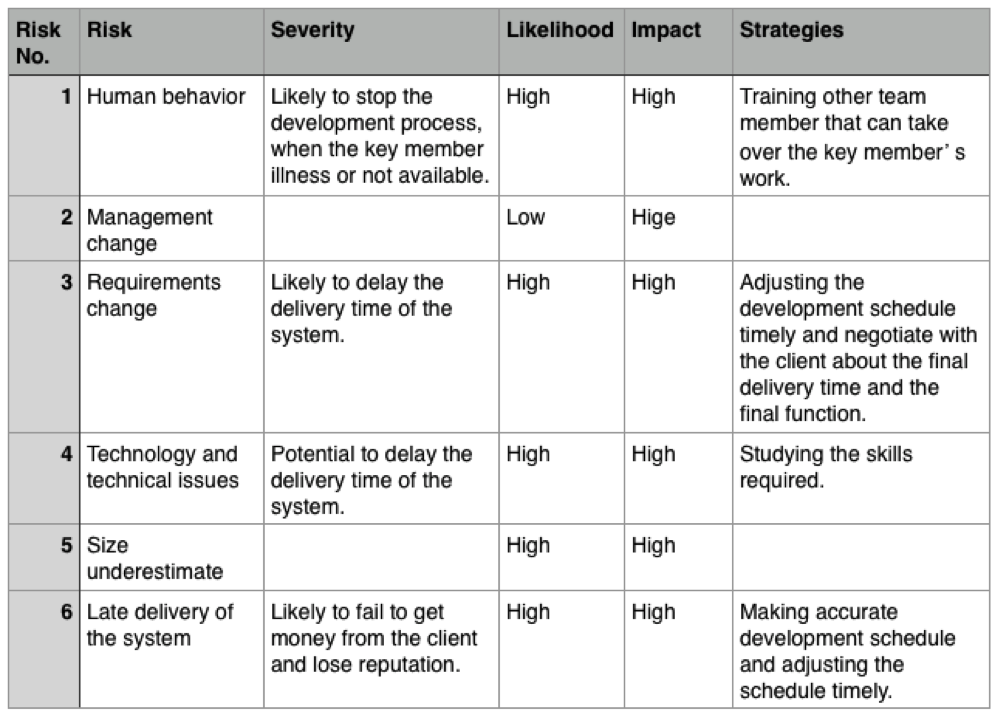
\includegraphics[height=4.5in]{RIA.png}
\caption[Risk Identification and Analysis]{Risk Identification and Analysis}
\end{figure}

%Here we insert our figure
\begin{figure}[H]
\centering
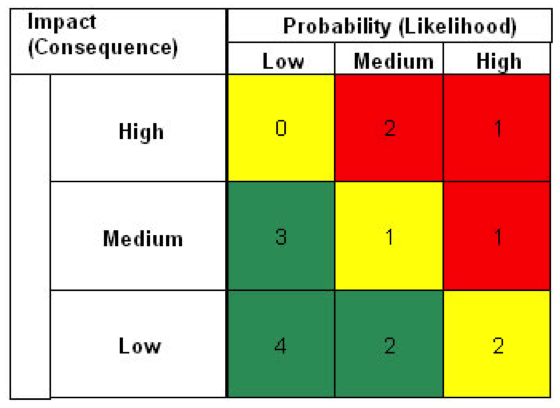
\includegraphics[height=3in]{RM.png}
\caption[Risk Matrix]{Risk Matrix}
\end{figure}

\textbf{Likelihood}
\begin{itemize}
\item { High - }More than 50\% probability of occurrence.
\item { Medium - }Between 25\% and 50\% probability of occurrence.
\item { Low - }Less than 25\% probability of occurrence
\end{itemize}

\textbf{Impact}
\begin{itemize}
\item { High - }Risk that will greatly impact project cost, project schedule and performance, if it occurs.
\item { Medium - }Risk that will slightly impact project cost, project schedule and performance, if it occurs.
\item { Low - }Risk that will little impact project cost, project schedule and performance, if it occurs.
\end{itemize}

\subsection{Risk Monitoring and Review}
Each identified risk will be monitoring and reviewed during the project scope. Risks will be listed top risks will be maintained by the project team. Requirements change may accompany with new risks, as a result, all the requirements change will be analysed for their possible to the project risks.
\newpage

%section6
\section{Process model}
AS the Mesa Mapping Robot project has low requirements volatility, short time of development and short release schedule. The software process model used in this project is component-based development.

%Here we insert our figure
\begin{figure}[H]
\centering
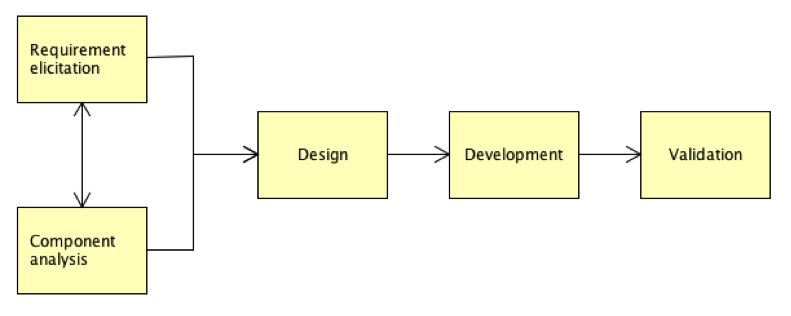
\includegraphics[height=2in]{PM.png}
\caption[Component-based Process Model]{Component-based Process Model}
\end{figure}

\textbf{Development Process}
\begin{itemize}
\item {Requirement elicitation and component analysis until week 5. }
\item {System design until week 6. }
\item {System development until week 10. }
\item {System validation until week 12. }
\end{itemize}
\newpage

%section7
\section{Work plan}
\subsection{Work activities}
%%Put the table here
\begin{tabular} 
	 {|p{1.2cm}|p{5cm}|p{1.4cm}|p{1.4cm}|p{1.2cm}|p{4cm}|}
\hline
{Task No} & {Task Name} & {Start Date} & {End Date} & {Duration} & {Assign to}\\
\hline
\textbf{T1} & \textbf{Intro to Project} & \textbf{03/08/15} & \textbf{21/08/15} & \textbf{21d} & \textbf{All members} \\
\hline
{}&{Requirements Gathering} & {03/08/15} & {14/08/15} & {14d} & {All members}\\
\hline
{T2} &{Repository} & {10/08/15}&{11/08/15}&{2d} & {Luo Yawen}\\
\hline
{} &{Google Drive} & {10/08/15}&{10/08/15}&{1d}&{Luo Yawen}\\
\hline
{} &{Group SVN} & {11/08/15}&{11/08/15}&{1d}&{Luo Yawen}\\
\hline
{T3} &{Poster} & {07/08/15}&{13/08/15}&{7d}&{Yang Jiajun} \\
\hline
{T4} &{Week 3 Meeting - requirements elicitation} & {10/08/15}&{14/08/15}&{3d}&{Zhang Yun}\\
\hline
{} &{Group Meeting} & {10/08/15}&{10/08/15}&{1d}&{Zhang Yun}\\
\hline
{} &{Client Meeting} & {11/08/15}&{11/08/15}&{1d}&{Zhang Yun} \\
\hline
{} &{Group Meeting} & {14/08/15}&{14/08/15}&{1d}&{Zhang Yun}\\
\hline
{T5} &{Week 4 Meeting - requirements elicitation \& milestone} & {17/08/15}&{21/08/15}&{3d}&{Luo Yawen}\\
\hline
{} &{Group Meeting} & {17/08/15}&{17/08/15}&{1d}&{Luo Yawen}\\
\hline
{} &{Client Meeting} & {18/08/15}&{18/08/15}&{1d}&{Luo Yawen}\\
\hline
{} &{Group Meeting} & {21/08/15}&{21/08/15}&{1d}&{Luo Yawen}\\
\hline
\textbf{T6} &\textbf{SRS First Draft} & \textbf{17/08/15}&\textbf{26/08/15}&\textbf{11d}&\textbf{All members}\\
\hline
{} &{Introduction} & {17/08/15}&{17/08/15}&{1d}&{Zander Shaun Nathan}\\
\hline
{} &{Overall Description} & {18/08/15}&{18/08/15}&{1d}&{Zander Shaun Nathan}\\
\hline
{} &{User Requirement} & {19/08/15}&{19/08/15}&{2d}&{Yang Jiajun \& Wang Yuzhu}\\
\hline
{} &{System Feature} & {21/08/15}&{21/08/15}&{2d}&{Luo Yawen \& Zhang Yun} \\
\hline 
{} &{External Interface Requirement} & {22/08/15}&{22/08/15}&{1d}&{Wei Jingwen} \\
\hline 
{} &{Other Nonfunctional Requirement} & {23/08/15}&{23/08/15}&{1d}&{Wei Jingwen} \\
\hline 
{} &{Other Requirements} & {24/08/15}&{24/08/15}&{1d}&{Wei Jingwen} \\
\hline 
{} &{Merging and Submission} & {25/08/15}&{26/08/15}&{2d}&{Luo Yawen} \\
\hline 
\textbf{T7} &\textbf{GUI Prototype} & \textbf{22/08/15}&\textbf{30/08/15}&\textbf{8d}&\textbf{Wang Yuzhu}\\
\hline
{} &{Design GUI Prototype} & {22/08/15}&{30/08/15}&{8d}&{Wang Yuzhu}\\
\hline
{T8} &{Week 5 Meeting -  Present Poster \& GUI \& Milestone} & {24/08/15}&{28/08/15}&{3d}&{Wang Yuzhu} \\
\hline 
{} &{Group Meeting} & {24/08/15}&{24/08/15}&{1d}&{Wang Yuzhu} \\
\hline 
{} &{Client Meeting} & {25/08/15}&{25/08/15}&{1d}&{Wang Yuzhu} \\
\hline 
{} &{Group Meeting} & {28/08/15}&{28/08/15}&{1d}&{Wang Yuzhu} \\
\hline 
{T9} &{Modify} & {28/08/15}&{30/08/15}&{3d}&{Wang Yuzhu} \\
\hline
\textbf{T10} &\textbf{Basic Movement Demo} & \textbf{24/08/15}&\textbf{04/09/15}&\textbf{14d}&\textbf{Wei Jingwen}\\
\hline
{} &{Design Robot Movement Demo} & {24/08/15}&{31/08/15}&{7d}&{Wei Jingwen}\\
\hline
{T11} &{Week 6 Meeting - GUI Prototype \& Basic Movement Demo} & {31/08/15}&{04/09/15}&{3d}&{Wei Jingwen} \\
\hline 
{} &{Group Meeting} & {31/08/15}&{31/08/15}&{1d}&{Wei Jingwen} \\
\hline 
{} &{Client Meeting} & {01/09/15}&{01/09/15}&{1d}&{Wei Jingwen} \\
\hline 
{} &{Group Meeting} & {04/09/15}&{04/09/15}&{1d}&{Wei Jingwen} \\
\hline 
\textbf{T12} &\textbf{Test Communication Function} & \textbf{31/08/15}&\textbf{04/08/15}&\textbf{5d}&\textbf{Zhang Yun}\\
\hline
\textbf{T13} &\textbf{SPMP First Draft} & \textbf{01/09/15}&\textbf{09/09/15}&\textbf{9d}&\textbf{All Members}\\
\hline
{} &{Introduction} & {01/09/15}&{01/09/15}&{1d}&{Wang Yuzhu}\\
\hline
{} &{Project Organisation} & {02/09/15}&{02/09/15}&{1d}&{Wang Yuzhu} \\
\hline 
{} &{Risk management Plan} & {04/09/15}&{05/08/15}&{2d}&{Wang Yuzhu} \\
\hline 
{} &{Process Model} & {05/09/15}&{05/09/15}&{1d}&{Wang Yuzhu} \\
\hline 
{} &{Work Plan} & {06/09/15}&{06/09/15}&{1d}&{Luo Yawen} \\
\hline 
{} &{Supporting Plans} & {07/09/15}&{07/09/15}&{1d}&{Yang Jiajun} \\
\hline 
{} &{Merging and submission} & {08/09/15}&{09/09/15}&{2d}&{Luo Yawen} \\
\hline 
\end{tabular}
\newpage
%%%%
\begin{tabular} 
	  {|p{1.2cm}|p{5cm}|p{1.4cm}|p{1.4cm}|p{1.2cm}|p{4cm}|}
\hline
\textbf{T14} &\textbf{Sensor Detection Function} & \textbf{01/09/15}&\textbf{24/09/15}&\textbf{24d}&\textbf{Wei Jingwen \& Zhang Yun}\\
\hline
{} &{Creating} &  {01/09/15}&{17/09/15}&{17d}&{Wei Jingwen \& Zhang Yun}\\
\hline
{} &{Testing} &  {18/09/15}&{24/09/15}&{7d}&{Wei Jingwen \& Zhang Yun} \\
\hline 
\textbf{T15} &\textbf{Manual Auto Switch Function} & \textbf{01/09/15}&\textbf{24/09/15}&\textbf{24d}&\textbf{Wei Jingwen \& Zhang Yun}\\
\hline
{} &{Creating} &  {01/09/15}&{17/09/15}&{17d}&{Wei Jingwen \& Zhang Yun}\\
\hline
{} &{Testing} & {18/09/15}&{24/09/15}&{7d}&{Wei Jingwen \& Zhang Yun} \\
\hline 
\textbf{T16} &\textbf{Week 7 Meeting - SRS Critique \& Milestone 1 Freeze} & \textbf{07/09/15}&\textbf{11/09/15}&\textbf{3d}&\textbf{Yang Jiajun} \\
\hline 
{} &{Group Meeting} &  {07/09/15}&{07/09/15}&{1d}&{Yang Jiajun} \\
\hline 
{} &{Client Meeting} &  {08/09/15}&{08/09/15}&{1d}&{Yang Jiajun} \\
\hline 
{} &{Group Meeting} &  {11/09/15}&{11/09/15}&{1d}&{Yang Jiajun} \\
\hline 
\textbf{T17} &\textbf{Week 8 Meeting - Milestone 2 Freeze} & \textbf{14/09/15}&\textbf{18/09/15}&\textbf{3d}&\textbf{Zander Shaun Nathan} \\
\hline 
{} &{Group Meeting} &  {14/09/15}&{14/09/15}&{1d}&{Zander Shaun Nathan} \\
\hline 
{} &{Client Meeting} &  {15/09/15}&{15/09/15}&{1d}&{Zander Shaun Nathan} \\
\hline 
{} &{Group Meeting} &  {18/09/15}&{19/09/15}&{1d}&{Zander Shaun Nathan} \\
\hline 
\textbf{T18} &\textbf{DTD} & \textbf{14/09/15}&\textbf{01/10/15}&\textbf{19d}&\textbf{Wei Jingwen \& Zhang Yun}\\
\hline
{} &{Creating} &  {14/09/15}&{18/09/15}&{10d}&{Wei Jingwen \& Zhang Yun}\\
\hline
{} &{Testing} &  {19/09/15}&{01/10/15}&{9d}&{Wei Jingwen \& Zhang Yun} \\
\hline 
\textbf{T19} &\textbf{Mapping} & \textbf{14/09/15}&\textbf{02/10/15}&\textbf{20d}&\textbf{Wei Jingwen \& Zhang Yun}\\
\hline
{} &{Mapping Loading} & {14/09/15}&{18/09/15}&{10d}&{Wei Jingwen \& Zhang Yun}\\
\hline
{} &{Testing} & {19/09/15}&{02/10/15}&{10d}&{Wei Jingwen \& Zhang Yun} \\
\hline 
\textbf{T20} &\textbf{SDD First Draft} & \textbf{25/09/15}&\textbf{06/10/15}&\textbf{13d}&\textbf{All members}\\
\hline
{} &{Introduction} & {25/09/15}& {25/09/15}&{1d}&{Luo Yawen}\\
\hline
{} &{System Overview} &{26/09/15}& {26/09/15}&{1d}&{Luo Yawen} \\
\hline 
{} &{System Architecture and Components } & {27/09/15}& {29/09/15}&{3d}&{Yang Jiajun}\\
\hline
{} &{Data Design} & {29/09/15}& {30/09/15}&{2d}&{Yang Jiajun} \\
\hline 
{} &{Design Details} &{30/09/15}&{02/10/15}&{3d}&{Wang Yuzhu}\\
\hline
{} &{Human Interface Design} & {02/10/15}&{04/10/15}&{3d}&{Wang Yuzhu} \\
\hline 
{} &{Merging and submission} & {05/10/15}&{06/10/15}&{2d}&{Luo Yawen} \\
\hline 
\textbf{T21} &\textbf{Week 9 Meeting - SPMP Critique \& Setting of mystery presentation topic \& Progress report} & \textbf {05/10/15}&\textbf {09/10/15}&\textbf{3d}&\textbf{Zhang Yun} \\
\hline 
{} &{Group Meeting} & {05/10/15}&{05/10/15}&{1d}&{Zhang Yun} \\
\hline 
{} &{Client Meeting} & {06/10/15}&{06/10/15}&{1d}&{Zhang Yun} \\
\hline 
{} &{Group Meeting} & {09/10/15}&{09/10/15}&{1d}&{Zhang Yun} \\
\hline 
\textbf{T22} &\textbf{Week 10 Meeting} & \textbf {12/10/15}&\textbf {16/10/15}&\textbf{3d}&\textbf{Wei Jingwen} \\
\hline 
{} &{Group Meeting} &{12/10/15}&{12/10/15}&{1d}&{Wei Jingwen} \\
\hline 
{} &{Client Meeting} & {13/10/15}&{13/10/15}&{1d}&{Wei Jingwen} \\
\hline 
{} &{Group Meeting} & {16/10/15}&{16/10/15}&{1d}&{Wei Jingwen} \\
\hline 
\textbf{T23} &\textbf{Week 11 Meeting - SDD Critique \& Mystery presentation topic \& Progress report} & \textbf {19/10/15}&\textbf {23/10/15}&\textbf{3d}&\textbf{Yang Jiajun} \\
\hline 
{} &{Group Meeting} & {19/10/15}&{19/10/15}&{1d}&{Yang Jiajun} \\
\hline 
{} &{Client Meeting} & {20/10/15}&{20/10/15}&{1d}&{Yang Jiajun} \\
\hline 
{} &{Group Meeting} & {23/10/15}&{23/10/15}&{1d}&{Yang Jiajun} \\
\hline 
\textbf{T24} &\textbf{Checking and Testing all Functions} & \textbf {15/10/15}&\textbf {25/10/15}&\textbf{10d}&\textbf{All members}\\
\hline 
\textbf{T25} &\textbf{Software Freeze} & \textbf {19/10/15}&\textbf {25/10/15}&\textbf{5d}&\textbf{All members}\\
\hline 
\textbf{T26} &\textbf{Final Presentation} & \textbf {02/11/15}&\textbf {06/11/15}&\textbf{7d}&\textbf{All Members}\\
\hline 
\textbf{T27} &\textbf{Meeting Minutes} & \textbf {11/08/15}&\textbf {20/10/15}&\textbf{32d}&\textbf{Zander Shaun Nathan \newline Wang Yuzhu}\\
\hline 
\textbf{T27} &\textbf{Agenda} & \textbf {11/08/15}&\textbf{20/10/15}&\textbf{32d}&\textbf{All members}\\
\hline 
\end{tabular}


\subsection{Milestones}
\subsubsection{Group Milestones}
\begin{itemize}
\item {\bfseries GM01 (due week 9)}\\
1: Robot Movement - Forward, back, left and right\\
2: Colour and distance sensor\\
3: GUI Prototype\\
4: Software Design Document (SDD) Draft\\
5: Software Project Management Plan (SPMP) Draft\\

\item {\bfseries GM02 (due week 10)}\\
1: The colour sensor, the movement range should be inside the boundary.\\
2: Let robot knows where the boundary is.\\
3: To combine the robot and GUI\\
4: To build the coordinate system\\
\end{itemize}

\subsubsection{Other Internal Milestones}
\begin{itemize}
\item {\bfseries M1} \\
1: GUI Design in paper- week 5\\
2: Robot Movement Demo - week 6\\
3: SRS draft - week 5
4: SPMP draft - week 7

\item {\bfseries M2}\\
1: GUI Prototype in the robot\\
2: Robot Movement accurate within one degree margin of error.\\
3: SDD draft - week 9\\
4: Through turning the arm, the robot can detect the boundary and stop emergency.\\
5: The robot can detect the colour accurately.\\
6: Through ultrasonic sensor, the robot can detect the obstacle.

\item {\bfseries M3}\\
1:To initial the map, through the robot walks along the boundary one rotation and detects the origin of coordinate.\\
2: Through scanning the map, the robot detects the coordinate of colours.\\
3: The robot detects obstacles and avoids them.\\
4: The robot detects NGZ and avoids it.\\
5: User Manual\\
6: Testing report\\
7: Saving and Loading map.\\

\end{itemize}
\newpage

\subsection{Schedule allocation}
This project is starting at the beginning of August and will be completed at the end of October. Form the schedule charts below, you can see details of our group process. Our group have a meeting with client and two meetings within group weekly. We do the task step by step and complete on time.

%Here we insert our figure
\begin{figure}[H]
\centering
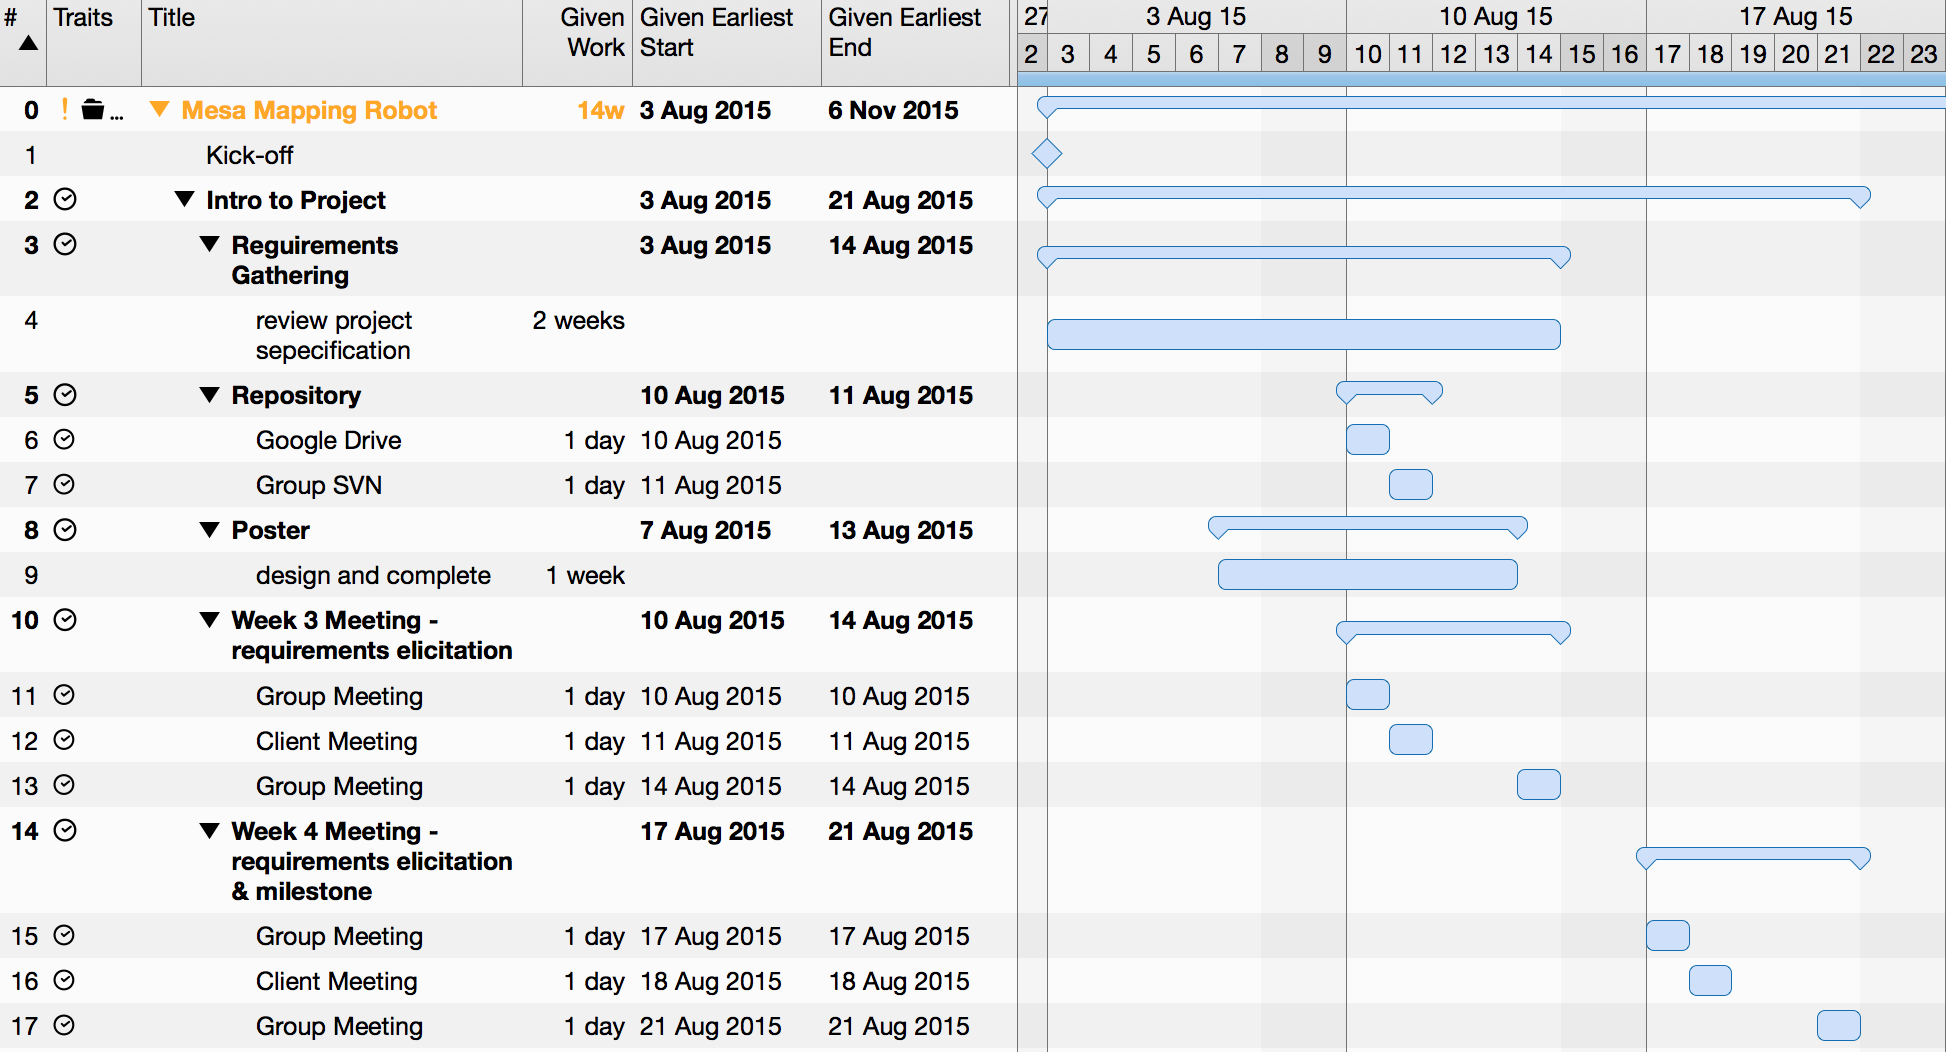
\includegraphics[height=3.5in]{SA1.png}
\end{figure}

\begin{figure}[H]
\centering
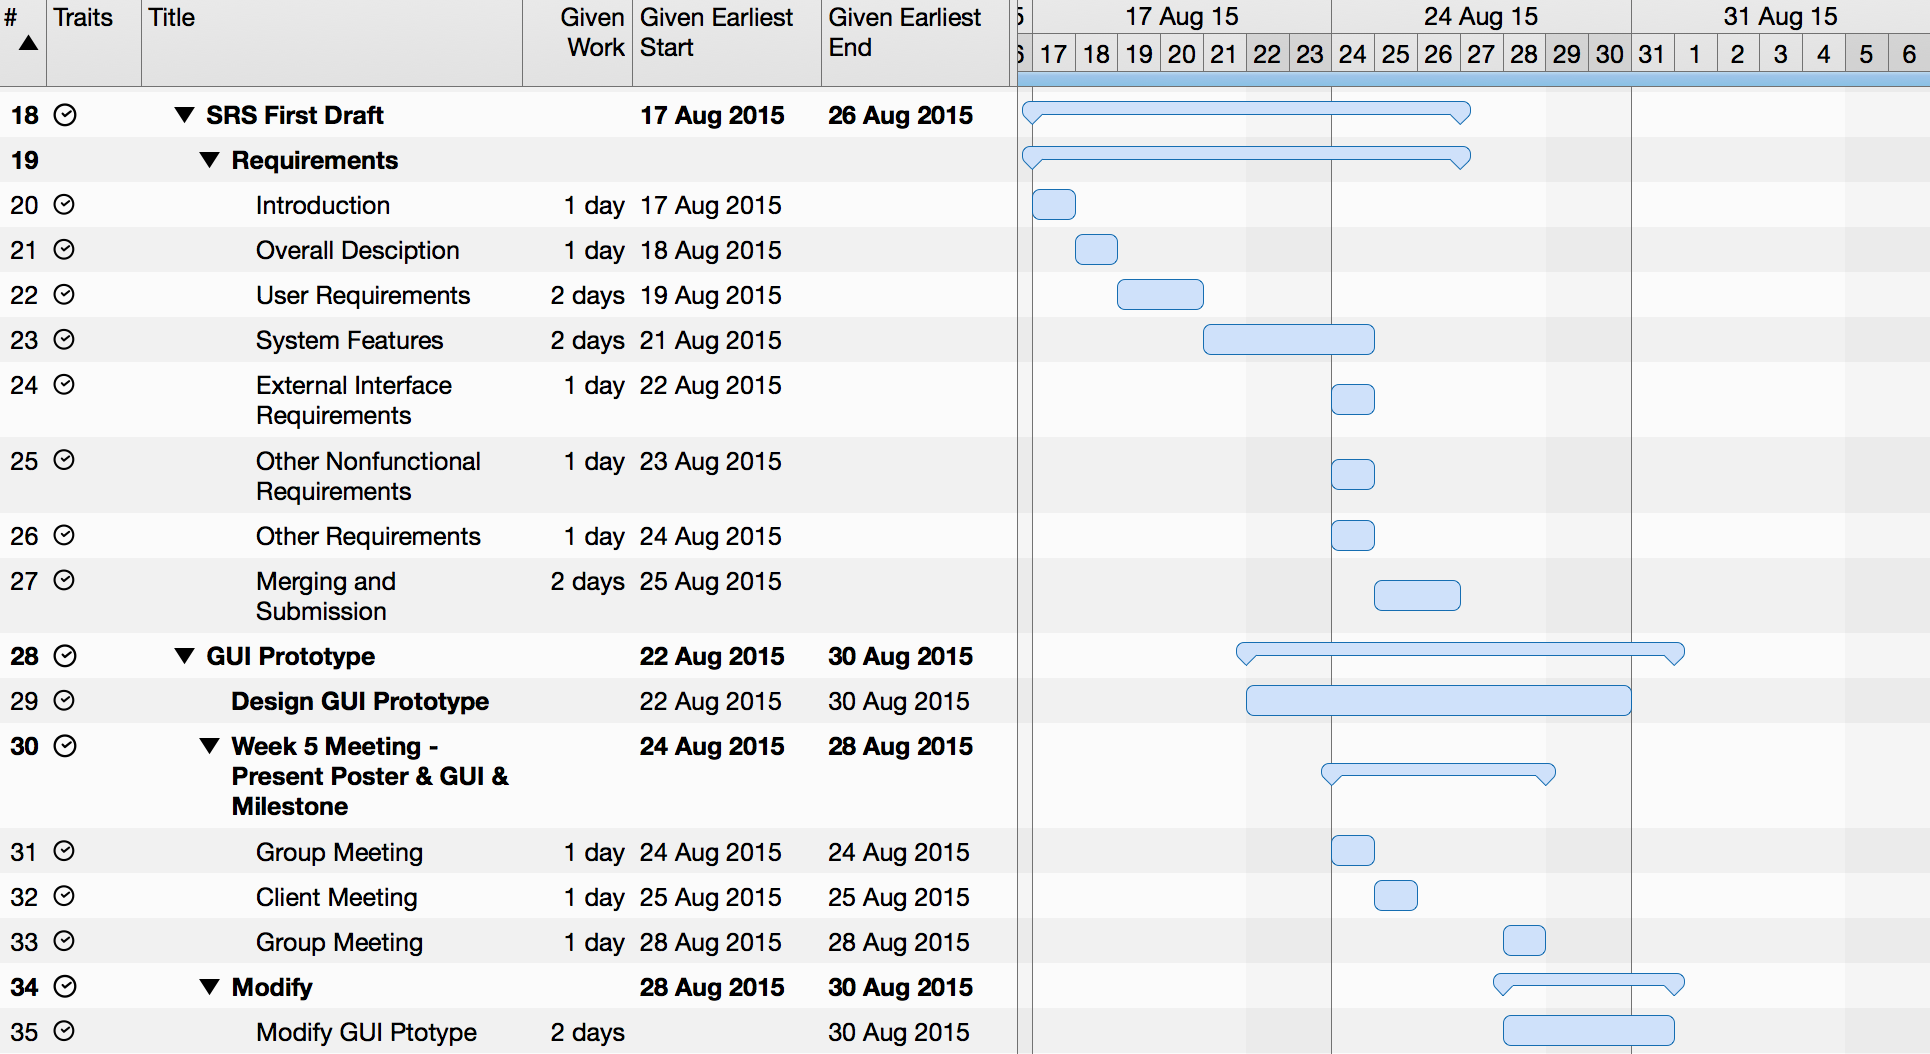
\includegraphics[height=3.5in]{SA2.png}
\end{figure}

\begin{figure}[H]
\centering
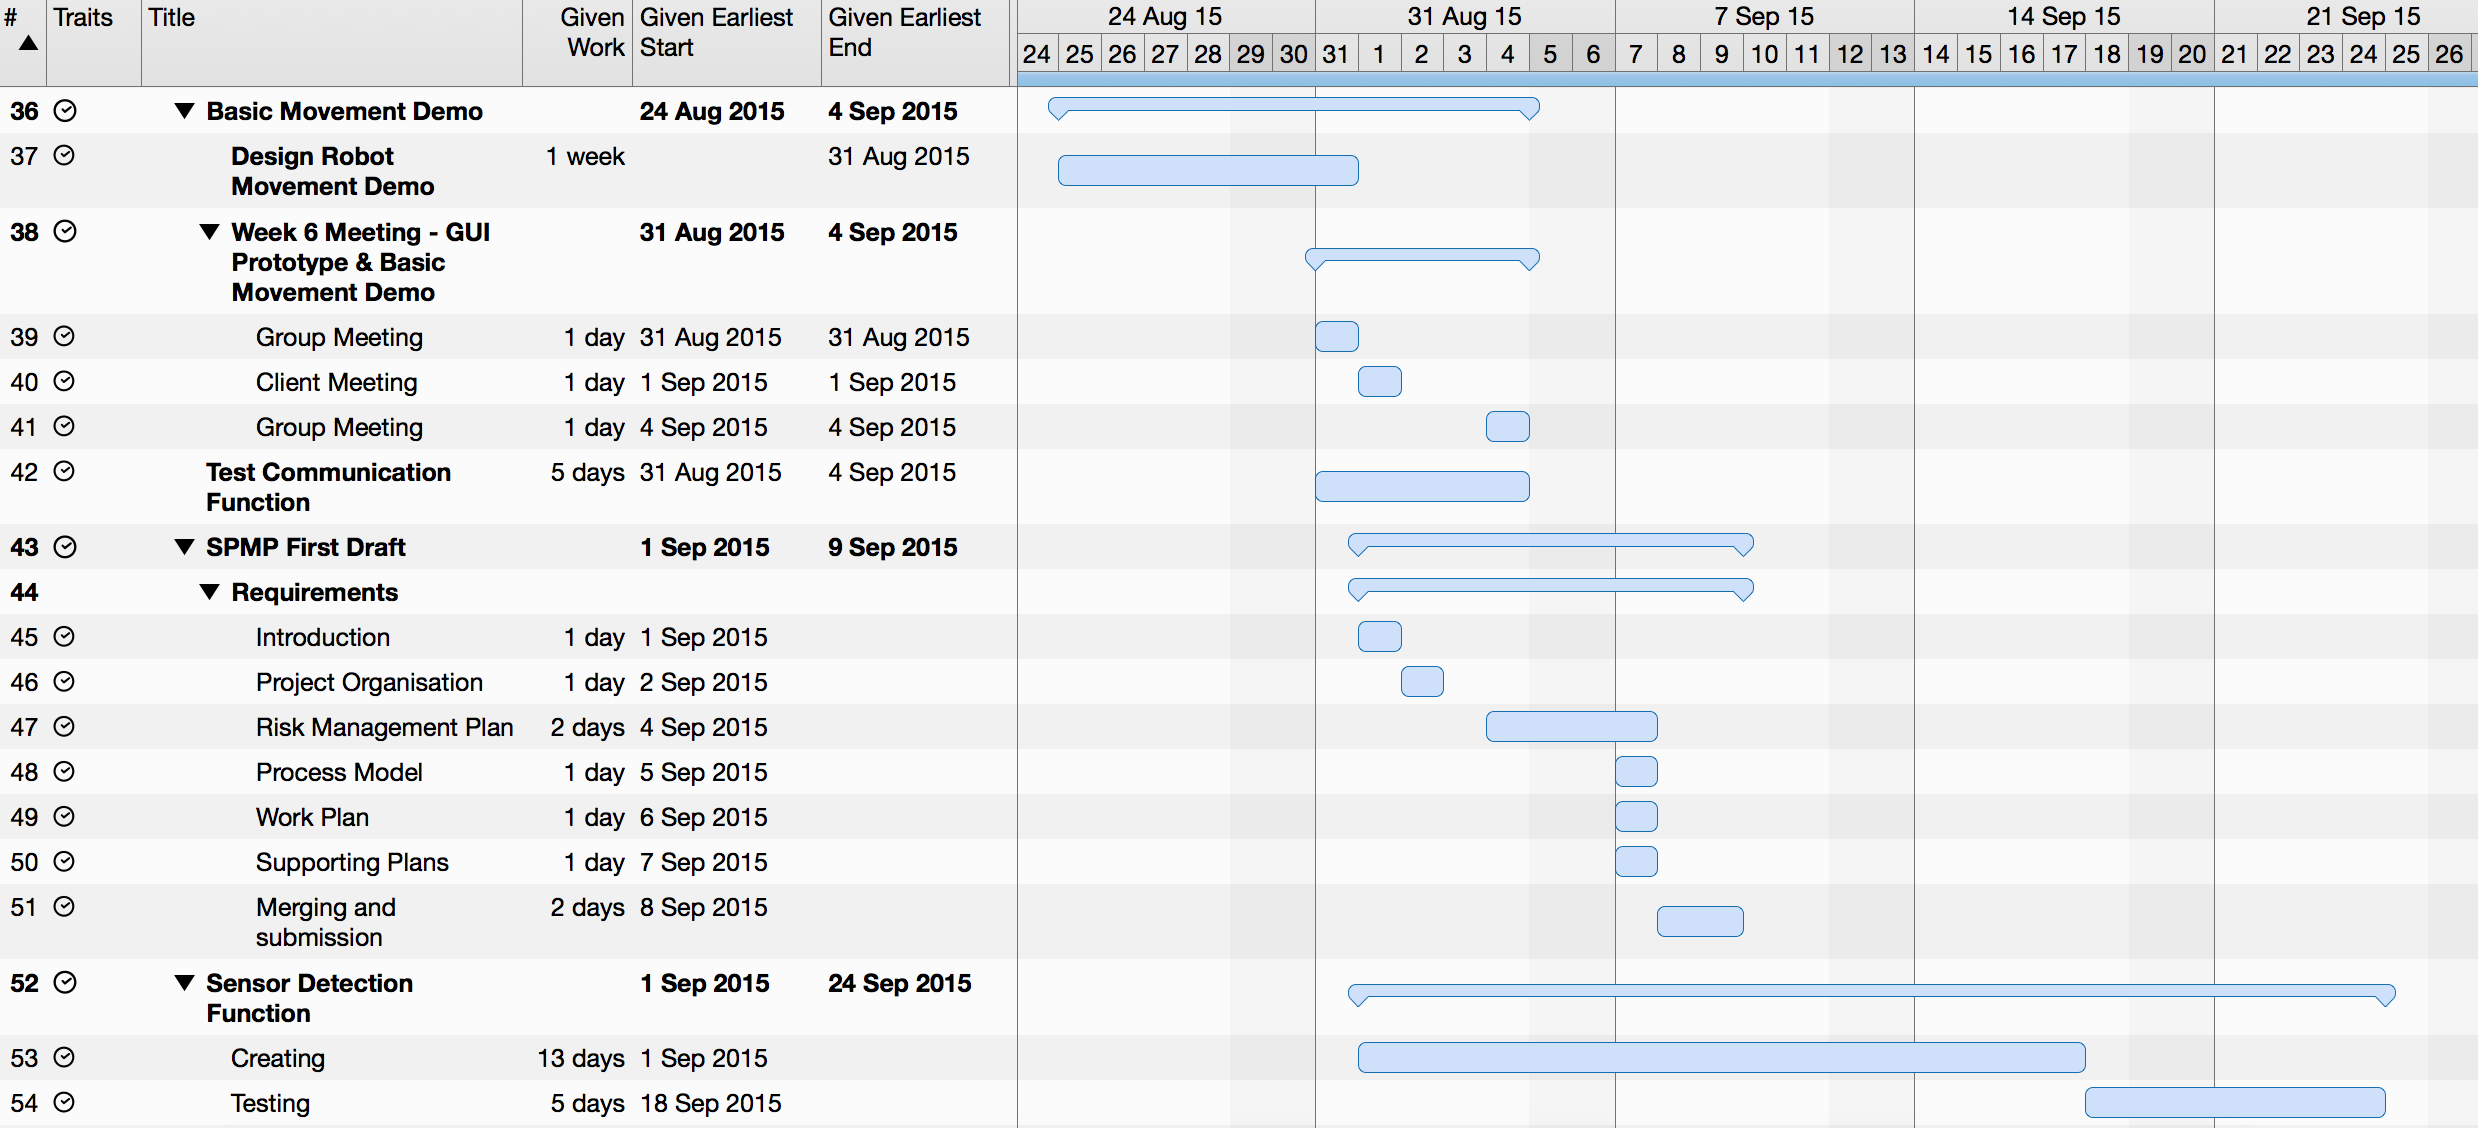
\includegraphics[height=3in]{SA3.png}
\end{figure}

\begin{figure}[H]
\centering
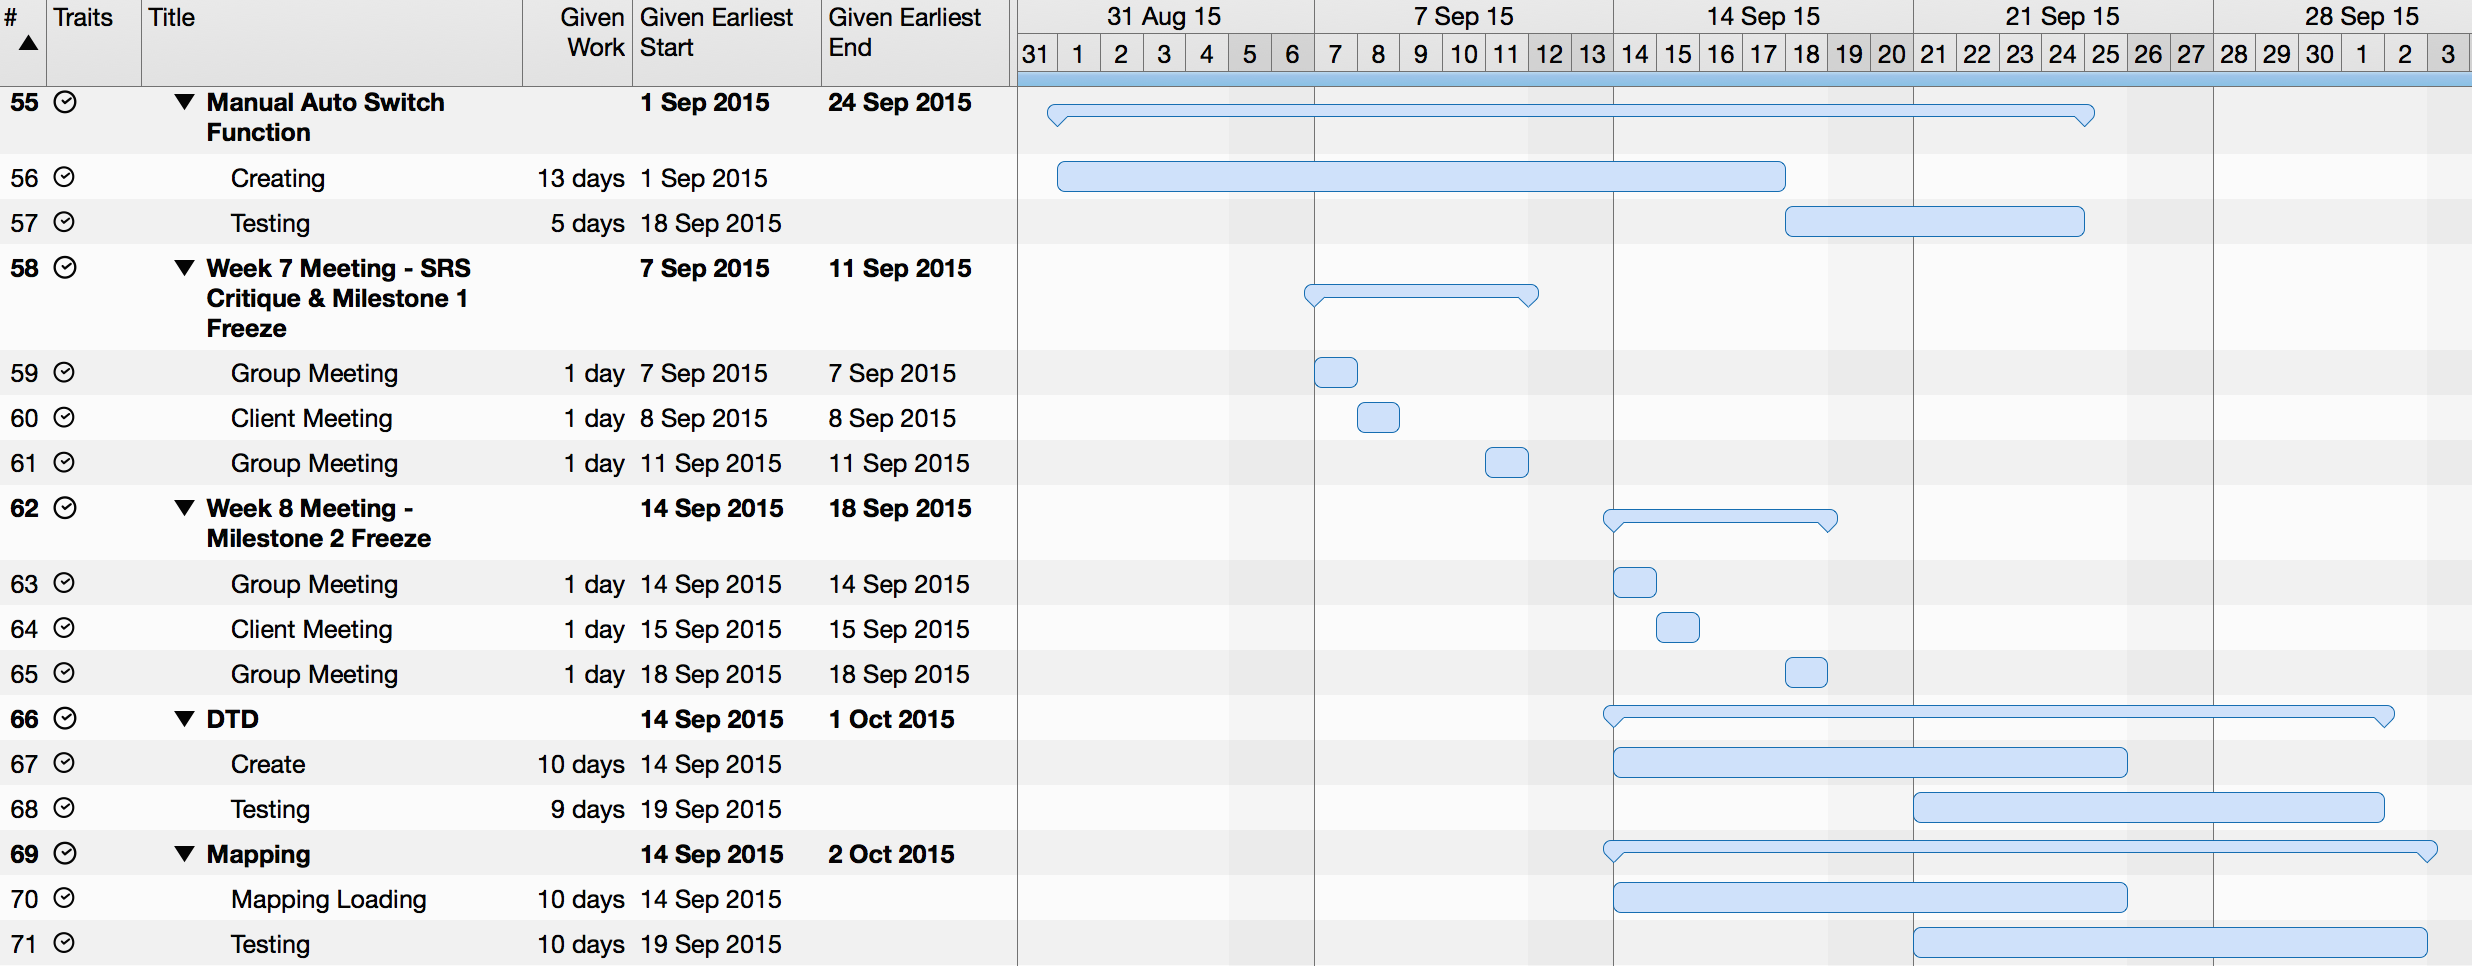
\includegraphics[height=2.6in]{SA4.png}
\end{figure}

\begin{figure}[H]
\centering
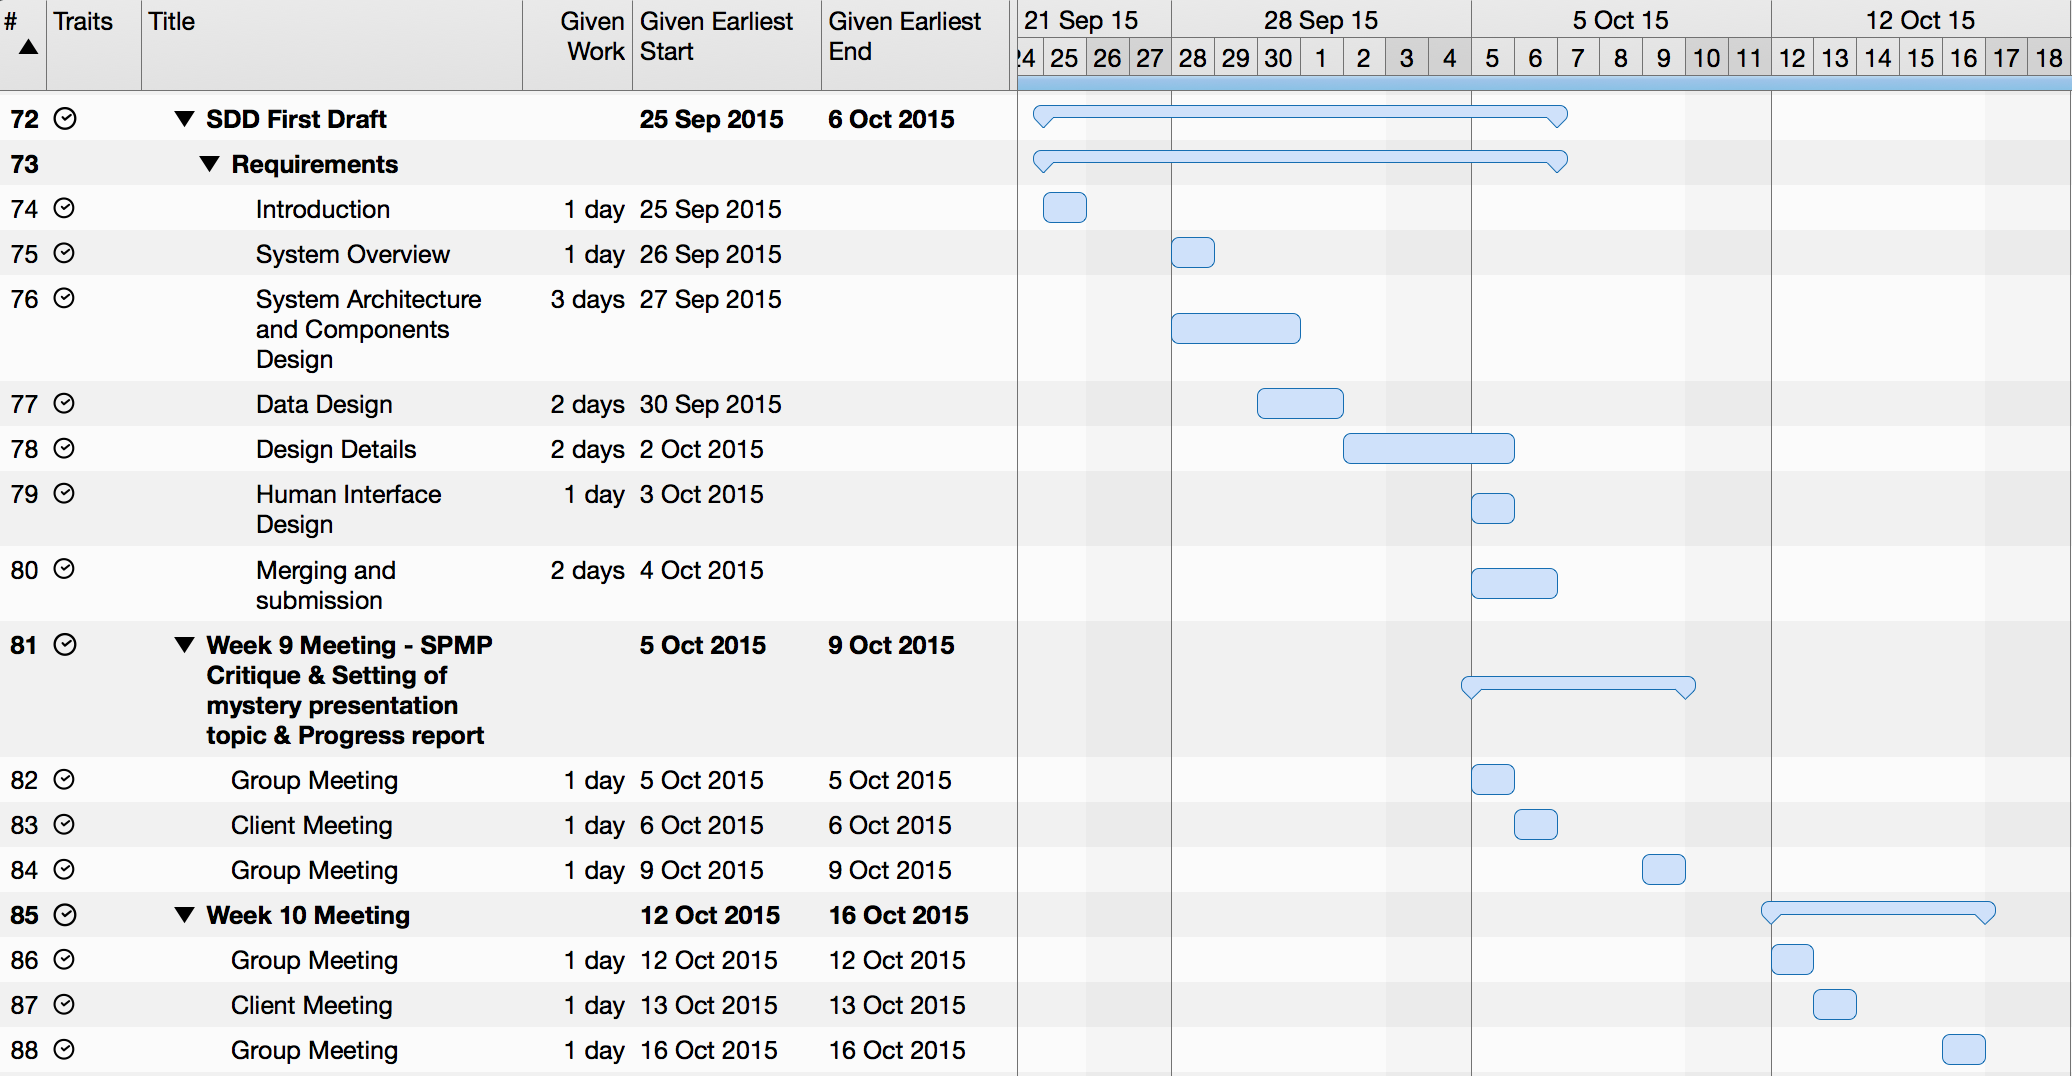
\includegraphics[height=3.3in]{SA5.png}
\end{figure}

\begin{figure}[H]
\centering
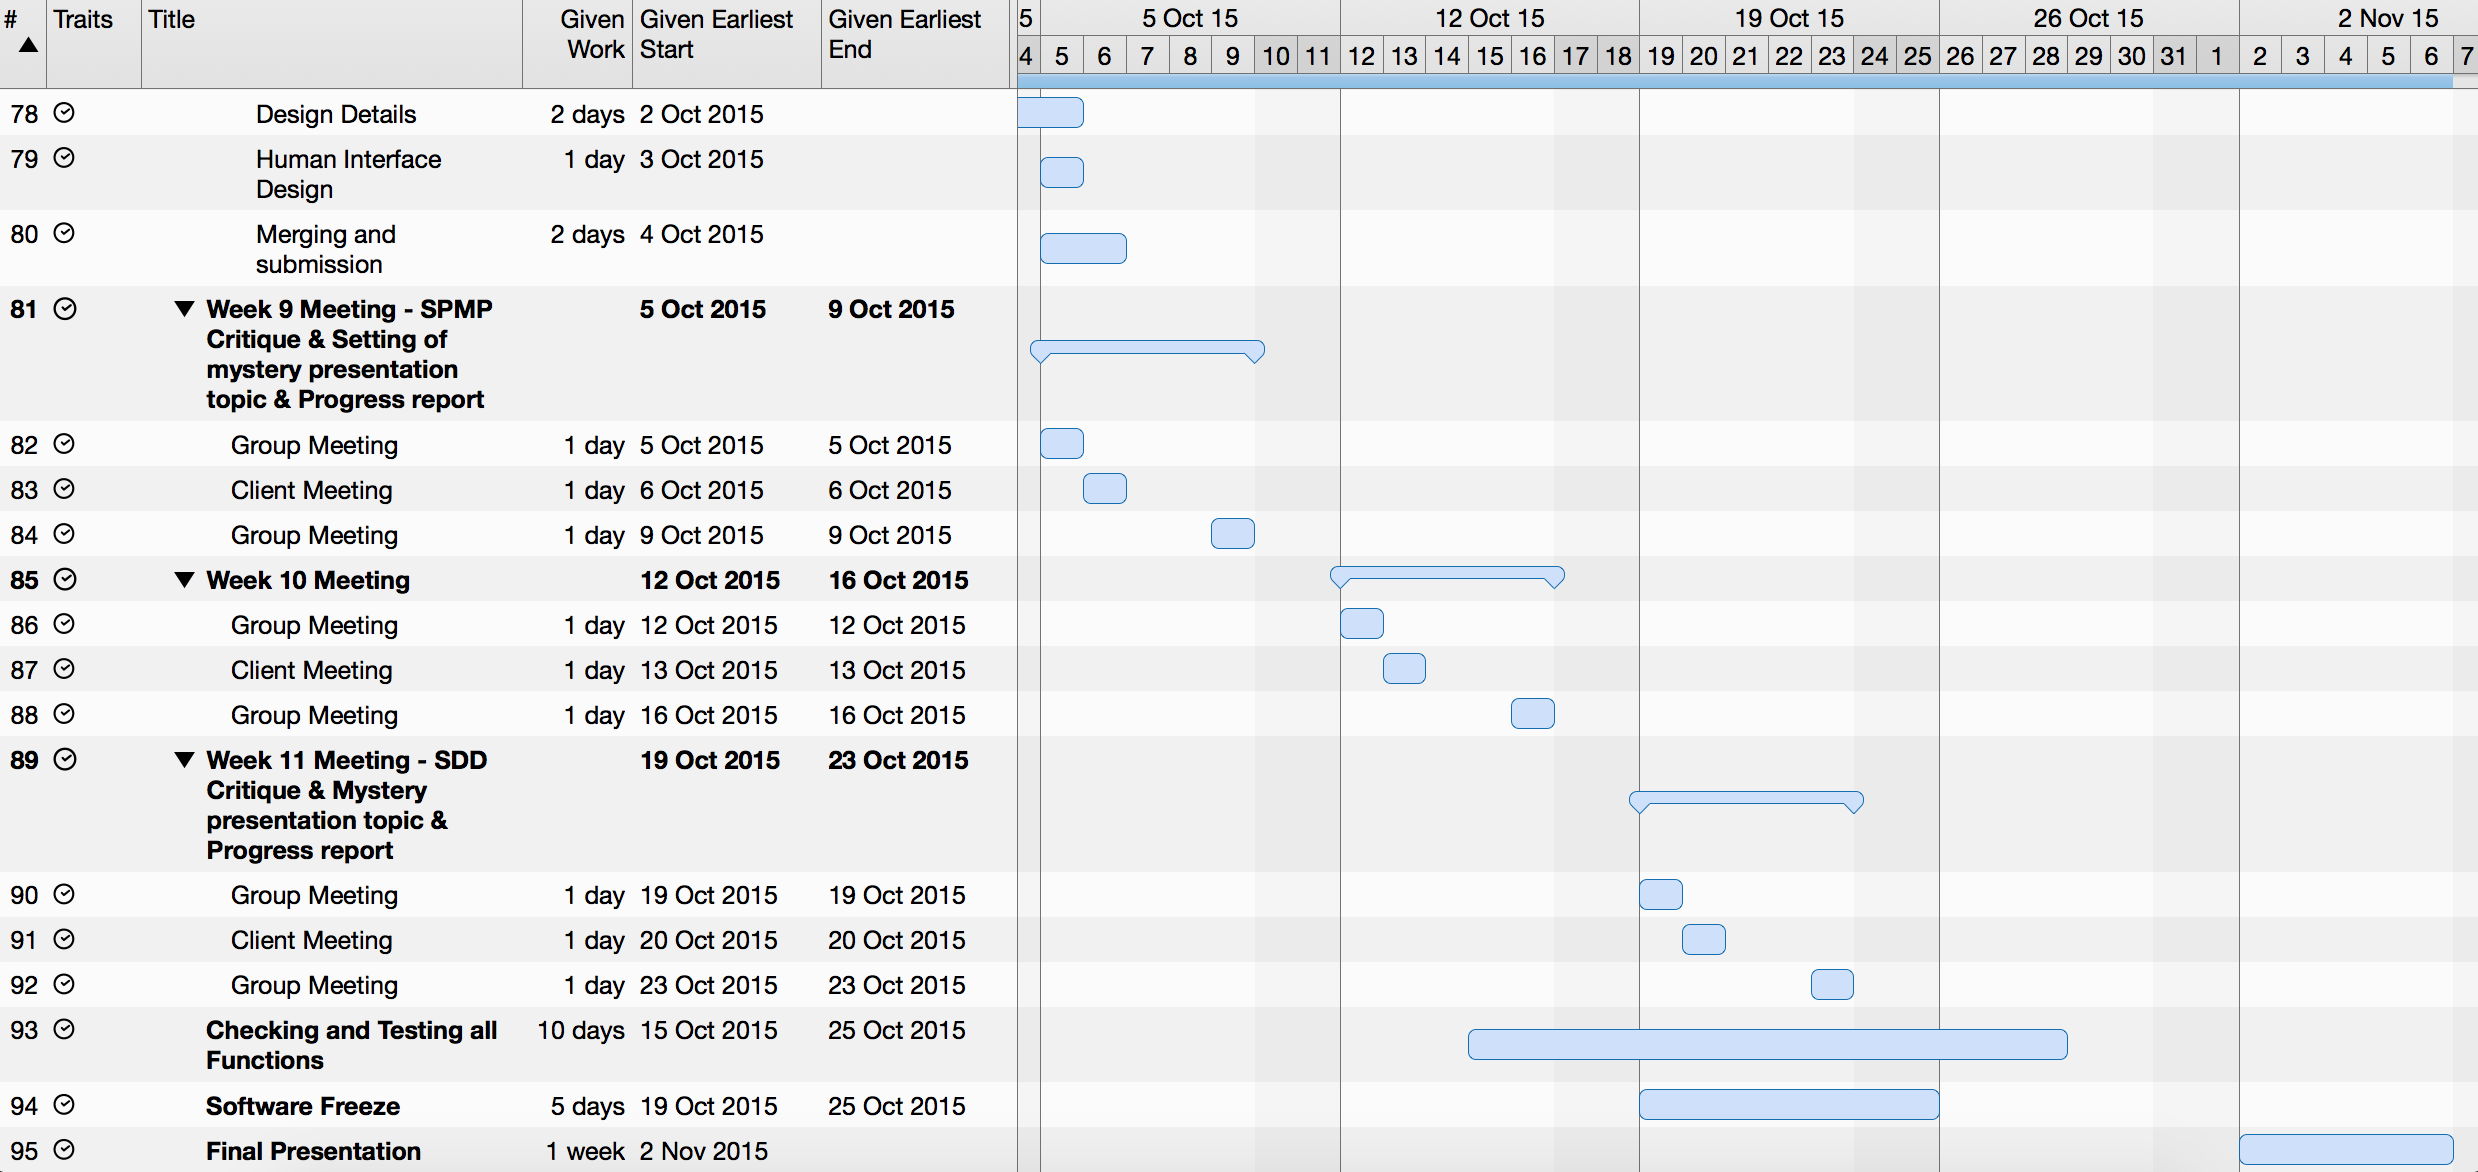
\includegraphics[height=3in]{SA6.png}
\end{figure}

\subsection{Resource allocation}
We allocate all tasks evenly based on each member's skills and what they are good at, and each member should do their tasks on time based on the work activities (section 7.1). If there is any change they should let project manager know in advance.
\newpage

%section8
\section{Supporting Plans}
For this project, there are three major supporting plans including configuration management plan, documentation plan and quality assurance plan.

\subsection{Configuration management plan}
In this project, the configuration items will uniquely be identified through three aspects, including product, document and develop tool. First, the product aspect contains the hardware, software and data. Second, the develop tools include the programming language and auxiliary tool. All detail of the product and develop tool would be described in several documents. In addition, the document part also contains risk management, user requirement etc. These documents would be identified by different titles. For different releases of a same document, they will be differentiated through version number.\\
\\
For our team, Google drive and SVN are utilised to store all the project documents, source code, milestone, meeting minute and agenda throughout the project lifecycle. \\
\\
\textbf{Repository structure:}\\
For the repository structure of the project, it contains tags and trunk directories. Among them, the trunk file is composed of several substructures as follows:\\
\begin{itemize}
\item {\bfseries SRS:} including the drafts and final version of SRS.\\
\item {\bfseries SPMP:} including the drafts and final version of SPMP.\\
\item {\bfseries SDD:} including the drafts and final version of SDD.\\
\item {\bfseries User Manual:} including the drafts and final version of user manual.\\
\item {\bfseries Source code:} including all the source code of the project.\\
\item {\bfseries Meeting agenda:} including all the meeting agendas.\\
\item {\bfseries Meeting minutes:} including all the meeting minutes.\\
\item {\bfseries Milestone:} including drafts and final version of milestone.\\
\item {\bfseries Testing report:} including drafts and final version of milestone.\\
\item {\bfseries GUI-Prototype:} including several design prototypes of GUI.\\
\item {\bfseries Poster:} including the final deliverable poster.\\
\end{itemize}

\subsection{Documentation Plan}
For this project, it mainly contains five documents, namely SRS, SPMP, SDD, User Manual and Testing Report. In addition, meeting minutes and agenda are also important part during the project lifecycle. All the documents would be mainly completed and submitted by the document team. For each document, all members of document team will discuss and take responsibility for different parts. After completed, all contents will be collected and tidied. As for review part, each member of document team needs to review the whole document and then, discuss with other members for improving the documents.\\

\begin{itemize}
\item {\bfseries Meeting minutes and agenda:} \\
For each meeting, one member will be nominated as the chair to supervise the whole meeting. What is more, the agenda should be prepared before the meeting by the chair. In addition, another member of our team will be the secretary to record then meeting minutes during the meeting. If necessary, video should be recorded by the secretary.\\

\item {\bfseries SRS:} \\
Identify the robot whose software requirements are specified in this document, including the revision or release number. Describe the scope of the project, such as overall description, system features and external interface requirements. The GUI prototype design was also provided in this document.\\

\item {\bfseries SPMP:} \\
The SPMP refers to the purpose and scope of the project to be delivered. Briefly summarise what is to be delivered, as well as what isn't going to be delivered. Project organisation and risk management are also provided in this document. In addition, it also identify the supporting plans such as configuration management plan and documentation plan to ensure the processing of the project.\\

\item {\bfseries SDD:}\\
Identify the context of the project; explain what the robot does (and what does not, if necessary). Describe data design, system architecture and components design. The description in this document should be consistent with the SRS.\\

\item {\bfseries User Manual:}\\
The user manual is designed for end users. All the functions of the robot will be identified in this document. Additionally, features, constraints and attentions of the robot will be displayed as well.\\

\item {\bfseries Testing report:}\\
The testing report should include the testing summary, assessment and result of the robot project. If possible, recommendations of any improvements in the design, operation, or future testing of the robot could be displayed.\\
\end{itemize}
\newpage

\subsection{Quality assurance plan}
For this project, we combined the waterfall model with the spiral model for the whole development lifecycle. First, for the requirement analysis stage, each of members classifies each requirement as functional, nonfunctional and others. Then, according to the client meeting we endow these requirements with different priority in the SRS document. In addition, we linked these different priority requirements with the system design in SDD. In other word, any subsystem or component will be cited with one or several requirements. This measure is utilised for ensuring all requirements could be realised and the high priority requirement could be focused on first. \\
\\
For this project, we have several strategies as follows to ensure the quality of the whole project.\\

\begin{itemize}
\item {\bfseries Weekly review}\\
For each week all members will have an extra on Friday morning to review the progress and unsolved problem. In addition, we will generate a target outline of next week. \\

\item {\bfseries Verification and Validation Process}\\
For the robot project, all the requirement details will be identified through project specification and client meetings. After programming, several testing strategies will be conducted by lay people to ensure all the requirements are meet. Pertaining to the document aspect, all documents will be accomplished cooperatively. However, the review task will be approved separately for maximum improvement of the project.\\
\item {\bfseries Standards:}\\ 
All the document need to be write and submit in Latex, and the develop language is JAVA. In addition, the specific content of these documents should follow the template as provided in computer science forum.\\

\item {\bfseries Review and inspection process:}\\
For each function of the robot, if it is approved, all members will inspect and test it. If possible, the function will be displayed in the weekly client meeting for collecting suggestion from the client for further improvement.\\
\end{itemize}

\end{document}